\documentclass[11pt]{article}
\usepackage[margin=1in]{geometry}
\usepackage{amsmath,amssymb,amsthm,mathtools}
\usepackage{stmaryrd}
\usepackage[expansion=false]{microtype}
\usepackage{xcolor}
\usepackage{booktabs,tabularx,array}
\usepackage{enumitem}
\usepackage{listings}
\usepackage{tikz}
\usetikzlibrary{positioning,arrows.meta,fit,calc}
\usepackage[hidelinks]{hyperref}
\usepackage{mathpartir}

\theoremstyle{plain}
\newtheorem{proposition}{Proposition}[section]
\newtheorem{lemma}[proposition]{Lemma}
\theoremstyle{definition}
\newtheorem{definition}[proposition]{Definition}
\newtheorem{requirement}{Requirement}
\newtheorem{remark}[proposition]{Remark}
\newtheorem{obligation}{Obligation}
\newtheorem{decision}{Open decision}

\newcommand{\Camp}{CampF1R3}
\newcommand{\Mfin}{M_{\mathrm{fin}}}
\newcommand{\rr}{\rightharpoonup}
\newcommand{\Bag}{\mathsf{Bag}}
\newcommand{\dom}{\mathrm{dom}}
\newcommand{\lin}{\mathsf{lin}}
\newcommand{\pers}{\mathsf{pers}}
\newcommand{\Red}{\mathsf{Redex}}
\newcommand{\Qui}{\mathsf{Q}}
\newcommand{\fp}{\mathsf{fp}}
\newcommand{\sh}{\mathsf{sh}}
\newcommand{\MUST}{\textsc{must}}
\newcommand{\MUSTNOT}{\textsc{must not}}
\newcommand{\SHOULD}{\textsc{should}}
\newcommand{\MAY}{\textsc{may}}
\usepackage[htt]{hyphenat}
\newcommand{\code}[1]{\texttt{#1}}
\setlength{\emergencystretch}{3em}

\definecolor{kw}{RGB}{0,0,140}
\definecolor{cm}{RGB}{90,110,90}
\lstdefinelanguage{Rust}{
  keywords={as,break,const,continue,crate,else,enum,extern,false,fn,for,if,impl,in,let,loop,match,mod,move,mut,pub,ref,return,self,Self,static,struct,super,trait,true,type,unsafe,use,where,while,dyn,Option,Result,Some,None,Ok,Err,Vec,bool,u8,u16,u32,u64,u128,usize,i32},
  sensitive=true,
  comment=[l]{//},
  morecomment=[s]{/*}{*/},
  morestring=[b]",
}
\lstset{
  language=Rust,
  basicstyle=\ttfamily\small,
  keywordstyle=\color{kw},
  commentstyle=\color{cm}\itshape,
  columns=fullflexible,
  keepspaces=true,
  frame=single,
  framerule=0.3pt,
  rulecolor=\color{black!30},
  xleftmargin=4pt,xrightmargin=4pt,
  aboveskip=6pt,belowskip=6pt,
  breaklines=true,
  literate={->}{{$\to$}}1 {=>}{{$\Rightarrow$}}1
}
\title{\textbf{\Camp}\\[4pt]
\large A small, multi-threaded, WASM-portable in-memory tuple store\\ that serves as an RSpace\\[6pt]
\normalsize Specification, version 0.1 (draft for review)}
\author{Lucius Gregory Meredith\\
\small CEO, F1R3FLY.io, and Chief Science Officer, F1R3FLY Industries}
\date{17 September 2026}

\begin{document}
\maketitle

\begin{abstract}
\Camp{} is a small, highly performant, multi-threaded, in-memory key--value
database written in Rust, cross-compilable to WebAssembly, whose sole purpose is
to serve as an RSpace: the tuple store against which a rho calculus reducer
materialises sends and receives and from which it obtains communication events.
This document specifies \Camp{}'s semantics, data structures, operations,
concurrency protocol, determinism profiles, cost-accounting hooks, portability
constraints, public interface, and conformance regime. The semantics is taken from
the RSpace denotation of the rho calculus --- tables $T_K(R)=K\rr(\Mfin(R)\uplus
\Mfin([N]R))$, parallel composition as key-wise multiset union, reaction as the
zip of dual bags --- extended to the joins, patterns, persistence, peeks and
guards that the F1R3FLY reducer actually requires. The design lever is the
factoring of RSpace into a store on keys and a reflection on values: \Camp{} is
the store, parametric in its key object, its inner collection, and its matcher,
and it knows nothing about processes. Parsing and normalisation are out of scope
and are treated in a separate specification.
\end{abstract}

\tableofcontents

%======================================================================
\section{Introduction}\label{sec:intro}

The RSpace of \code{f1r3node-rust} (crate \code{rspace++}, branch
\code{feature/cost-accounted-rho}) is roughly 21\,000 lines of Rust, of which the
in-memory tuple store --- the part the reducer actually talks to during
evaluation --- is a few thousand. The remainder is the radix history trie, LMDB
persistence, the merger, and replay. The whole crate depends transitively on
\code{heed} (LMDB, C code), \code{tokio}, and \code{rayon}, and its hot paths
call \code{std::time::Instant::now}, which panics on
\code{wasm32-unknown-unknown}. None of that is required to be an RSpace.

\Camp{} is the RSpace with everything that is not the store removed. It is
specified here as a standalone crate family with three commitments:
\begin{enumerate}[nosep]
\item it is exactly the store monad together with the zip, generalised to what
      the reducer needs, and nothing else (Section~\ref{sec:semantics});
\item it runs unchanged on native targets and on WebAssembly, with or without
      threads (Section~\ref{sec:wasm});
\item it plugs into the existing reducer through the existing type parameters
      $C,P,A,K$ = \code{Par}, \code{BindPattern}, \code{ListParWithRandom},
      \code{TaggedContinuation}, so the \code{f1r3node} parser, normaliser and
      spatial matcher can be reused once they are extracted
      (Section~\ref{sec:integration}).
\end{enumerate}

\paragraph{Sources.}
\begin{itemize}[nosep]
\item Semantic basis: the RSpace denotation of \emph{Quoting is Colour-Swap}, \S5\\
      (\code{publications/denotational-semantics-for-rho/knot-rho.tex}).
\item Key-object polymorphism: \emph{Paths are Subspaces}\\
      (\code{publications/polymorphic-rspace/paths-subspaces.tex}).
\item Operational surface and storage variants: the approved FIP \emph{Reifying RSpaces}\\
      (\code{FIPs/approved/2025-09-26-Reifying-RSpaces}).
\item Interface to be served: \code{ISpace} and \code{Match} in \code{rspace++},
      \code{f1r3node-rust} commit \code{619beb4}.
\end{itemize}

%----------------------------------------------------------------------
\subsection{Goals}

\begin{description}[nosep,leftmargin=2.2em,style=nextline]
\item[G1 Small.] The core crate is at most about 3\,000 lines of non-test Rust
  and has no mandatory third-party dependency outside a short allowlist
  (Section~\ref{sec:deps}).
\item[G2 Fast.] The common operations --- a send or receive on a single channel
  that belongs to no join --- touch one shard, take one lock, perform no
  allocation beyond the stored record, and never hash or serialise a payload.
\item[G3 Multi-threaded.] Operations whose footprints are disjoint run in
  parallel; throughput on disjoint channels scales with the number of shards up to
  the number of hardware threads.
\item[G4 Portable.] The core builds for \code{wasm32-unknown-unknown} (single
  threaded), \code{wasm32-unknown-unknown} with atomics, and
  \code{wasm32-wasip1-threads}, with identical observable semantics.
\item[G5 Conformant.] Every operation preserves the quiescence invariant of
  Section~\ref{sec:semantics}, and the store is linearisable.
\item[G6 Reusable.] The store is generic in channel, pattern, datum and
  continuation types, and in the matcher, so the \code{f1r3node} types plug in
  without conversion.
\end{description}

\subsection{Non-goals}

\Camp{} does \emph{not} parse, normalise, substitute, or evaluate processes; it
does not run continuations; it does not persist to disk, maintain a history trie,
compute state roots compatible with \code{rspace++}, merge concurrent blocks,
gossip, or take part in consensus. It does not spawn threads: parallelism is
supplied by the caller. Vector-database channels and quantale semantics for
sequential processes (both discussed in the FIP) are out of scope for version~1.

\subsection{Conformance language}

The keywords \MUST, \MUSTNOT, \SHOULD{} and \MAY{} are used in the sense of
RFC~2119. Numbered \emph{Requirements} are normative. \emph{Remarks} are
explanatory. \emph{Obligations} are proof or validation tasks that the design
relies on but that this document does not discharge. \emph{Open decisions} are
choices deferred to review; each states the default this draft adopts.

%======================================================================
\section{Semantic model}\label{sec:semantics}

\subsection{The table, and why it is the specification}

In the RSpace denotation, a process modulo structural congruence is sent to a
table
\[
  T_K(R) \;=\; K \rr \big(\Mfin(R)\uplus\Mfin([N]R)\big),
\]
a finite partial map from keys to polarity-homogeneous bags: at each key either a
bag of output payloads or a bag of input continuations. Parallel composition is
key-wise multiset union $\uplus_K$, so the denotation is a commutative-monoid
homomorphism and the parallel laws of structural congruence hold as literal
equalities of tables. Reaction is \emph{eager}: a key carrying both polarities is
a redex, and firing it zips the two bags, applying each matched continuation to
the quoted payload. RSpace is the store monad $K\rr\Mfin(-)$ together with this
zip, presented as a distributive law --- a bialgebra.

Two facts from that account govern the whole of \Camp{}.

\begin{remark}[The factoring]\label{rem:factoring}
RSpace is a reflection structure on \emph{values} glued at the table to a store
monoid on \emph{keys}. Changing the key object, or the collection at each key,
leaves the reflection law untouched. \Camp{} implements only the store-and-zip
factor. Quoting and dereference are the caller's business, carried inside the
opaque types $C$, $A$ and $K$.
\end{remark}

\begin{remark}[No implicit interaction]\label{rem:noimplicit}
The store never reacts with itself. A reaction is triggered only by a cut: the
arrival of one send or one receive, co-located with the store. In \Camp{} every
mutating operation is exactly such a cut, and nothing else ever fires.
\end{remark}

\subsection{From tables to what the reducer needs}

The table above is single-channel, patternless and linear. The F1R3FLY reducer
needs five generalisations, each of which \Camp{} \MUST{} support:
\begin{enumerate}[nosep]
\item \textbf{joins} --- a receive listens on an ordered group of channels
      $g=(c_1,\dots,c_n)$ and fires only when every position is satisfied;
\item \textbf{patterns} --- a redex requires a successful match, not mere
      co-location;
\item \textbf{persistence} --- persistent sends and receives (\code{<=},
      replicated output), the store-level face of the $\mathbb N\cup\{\omega\}$
      completion forced by replication;
\item \textbf{peeks} --- positions of a join that read a datum without
      consuming it;
\item \textbf{guards} --- a \code{where} clause evaluated over all bindings of a
      join after spatial matching succeeds.
\end{enumerate}
With patterns, polarity homogeneity is no longer the normal-form condition: a
channel may legitimately hold both data and continuations that simply do not
match. The normal form becomes \emph{quiescence}, the ``no match remains''
invariant of the FIP.

\subsection{State}

Fix sets $C$ (channels, with decidable equality), $P$ (patterns), $A$ (data), and
$K$ (continuations), and a \emph{matcher} consisting of
\[
  m : P\times A \rr A \qquad\text{and}\qquad \gamma : K\times A^{*}\to\{\top,\bot\},
\]
where $m(p,a)$ is defined when $a$ matches $p$, returning the binding result, and
$\gamma$ is the guard. Let $\pi\in\{\lin,\pers\}$ be a persistence flag.

\begin{definition}[Records]
A \emph{datum} is $d=(a,\pi,h)$ with $a\in A$ and $h$ its content hash. A
\emph{waiting continuation} is $w=(\vec p,k,\pi,E,h)$ with
$\vec p=(p_1,\dots,p_n)\in P^n$, $k\in K$, and $E\subseteq\{1,\dots,n\}$ the peek
positions.
\end{definition}

\begin{definition}[Store state]\label{def:state}
A state is $\Sigma=(D,W,I)$ where
\[
  D : C\rr\Bag(\text{datum}),\qquad
  W,\ I : C^{+}\rr\Bag(\text{waiting continuation}),
\]
with $W$ the ordinary and $I$ the installed continuations, every continuation at
group $g$ having $|\vec p|=|g|$. The join index is derived, not stored
independently:
$J_\Sigma(c)=\{\,g\in\dom W\cup\dom I \mid c\in g\,\}$.
\end{definition}

For the bag instance, states form a commutative monoid under key-wise $\uplus$
with the empty state as unit, which is the table monoid of the source paper
extended by the group-keyed component.

\subsection{Redexes and quiescence}

\begin{definition}[Candidate]\label{def:candidate}
Let $w=(\vec p,k,\pi,E,h)$ wait at $g=(c_1,\dots,c_n)$. A \emph{candidate} for $w$
is a tuple of data occurrences $\vec d=(d_1,\dots,d_n)$ with $d_i$ an occurrence in
$D(c_i)$ such that
\begin{enumerate}[nosep]
\item occurrences are pairwise distinct (if $c_i=c_j$ with $i\neq j$, then
      $d_i$ and $d_j$ are different occurrences, though they may be equal
      values);
\item $b_i=m(p_i,a_i)$ is defined for every $i$;
\item $\gamma(k,\vec b)=\top$.
\end{enumerate}
$\Red(\Sigma)$ is the set of triples $(g,w,\vec d)$ with $\vec d$ a candidate for
$w$.
\end{definition}

\begin{definition}[Quiescence]
$\Sigma$ is \emph{quiescent}, $\Qui(\Sigma)$, when $\Red(\Sigma)=\varnothing$.
\end{definition}

\begin{requirement}[Quiescence invariant]\label{req:qui}
Every state observable between completed operations \MUST{} be quiescent with
respect to the configured matching strategy (Section~\ref{sec:matching}).
\end{requirement}

\subsection{Operations as cuts}\label{sec:opsem}

We write $\Sigma+_c d$ for $\Sigma$ with occurrence $d$ added to $D(c)$,
$\Sigma+_g w$ similarly, and $\Sigma-x$ for removal of an occurrence. A choice of
redex is delegated to an \emph{oracle} $\omega$ (Section~\ref{sec:determinism}):
this is precisely the pairing nondeterminism of the source paper, localised at
one cut.

\begin{definition}[Consumption of a redex]
For $(g,w,\vec d)$ with $w=(\vec p,k,\pi,E,h)$, set
\[
  \mathsf{fire}(\Sigma,g,w,\vec d) \;=\;
  \Sigma \;-\;\{\,w \mid \pi=\lin\,\}\;-\;
  \{\,d_i \mid d_i.\pi=\lin \text{ and } i\notin E\,\},
\]
returning the \emph{comm result}
$\kappa=(k,\ \pi,\ g,\ \vec p,\ (b_i,\,a_i,\,d_i.\pi)_{i})$: the continuation,
its persistence, the group, the patterns, and for each position the binding
result, the removed datum, and the datum's persistence.
\end{definition}

The three mutating operations are given by the following rules, each read on a
quiescent input state $\Sigma$.

\begin{mathpar}
\inferrule*[right=Produce-Store]
 {d=(a,\pi,h) \\ \nexists\,(g,w,\vec d)\in\Red(\Sigma+_c d)\ \text{using}\ d}
 {\mathsf{produce}(c,a,\pi):\ \Sigma \Longrightarrow \Sigma+_c d,\ \ \mathsf{None}}

\inferrule*[right=Produce-Comm]
 {d=(a,\pi,h) \\ (g,w,\vec d)=\omega\big(\{\,r\in\Red(\Sigma+_c d)\mid r\ \text{uses}\ d\,\}\big)}
 {\mathsf{produce}(c,a,\pi):\ \Sigma \Longrightarrow
  \mathsf{fire}(\Sigma+_c d,g,w,\vec d)\ominus d,\ \ \mathsf{Some}(\kappa)}

\inferrule*[right=Consume-Store]
 {w=(\vec p,k,\pi,E,h) \\ \nexists\ \text{candidate for}\ w\ \text{in}\ \Sigma}
 {\mathsf{consume}(g,\vec p,k,\pi,E):\ \Sigma \Longrightarrow \Sigma+_g w,\ \ \mathsf{None}}

\inferrule*[right=Consume-Comm]
 {w=(\vec p,k,\pi,E,h) \\ \vec d=\omega(\text{candidates for}\ w\ \text{in}\ \Sigma)}
 {\mathsf{consume}(g,\vec p,k,\pi,E):\ \Sigma \Longrightarrow
  \mathsf{fire}(\Sigma+_g w,g,w,\vec d)\ominus w,\ \ \mathsf{Some}(\kappa)}

\inferrule*[right=Install]
 {w=(\vec p,k,\pers,\varnothing,h) \\ \nexists\ \text{candidate for}\ w\ \text{in}\ \Sigma}
 {\mathsf{install}(g,\vec p,k):\ \Sigma \Longrightarrow \Sigma+^{I}_g w,\ \ \mathsf{None}}
\end{mathpar}

\noindent
Here $\Sigma\ominus x$ removes occurrence $x$ if it is still present (it may already
have been removed by $\mathsf{fire}$, or kept there as a peek).
The arriving record is \emph{never stored} when it reacts, even if persistent:
its persistence is honoured by the caller re-issuing it, exactly as \code{ISpace}
documents (``to make data stick, call produce until None''). \code{install} with
an existing candidate is an error (installation happens at start-up), and
installed continuations survive \code{clear} and checkpoint reversion.

\begin{proposition}[Operations preserve quiescence]\label{prop:qui}
If $\Qui(\Sigma)$ and $\mathsf{op}:\Sigma\Longrightarrow\Sigma'$ by any rule above,
with $\omega$ drawing from the complete candidate set, then $\Qui(\Sigma')$.
\end{proposition}
\begin{proof}
For the \textsc{Store} rules the premise says no redex of the extended state uses
the new record; any other redex would already be a redex of $\Sigma$. For the
\textsc{Comm} rules the new record is absent from $\Sigma'$, and $\Sigma'$ is
obtained from $\Sigma$ by removing occurrences only. Removing data or
continuations cannot create a candidate (candidacy is monotone in the bags: every
candidate of a sub-state is a candidate of the state), so any redex of $\Sigma'$
is a redex of $\Sigma$, contradicting $\Qui(\Sigma)$.
\end{proof}

\begin{remark}[Why the arriving record is not stored on reaction]
Proposition~\ref{prop:qui} depends on it. If a persistent arriving datum were
stored after reacting with one continuation, a second waiting continuation matching
the same datum would be a live redex in the resulting state. The re-issue
obligation is the price of keeping every operation a single cut, and is what lets
the store return at most one comm result per call.
\end{remark}

\begin{requirement}[Re-issue contract]\label{req:reissue}
A caller that receives $\mathsf{Some}(\kappa)$ from an operation whose arriving
record was persistent \MUST{} re-issue that operation after scheduling the
continuation, until it returns $\mathsf{None}$, if it wants the record to
persist. \Camp{} \MUSTNOT{} re-issue on the caller's behalf.
\end{requirement}

\subsection{Correspondence with the calculus}

Let $\llbracket\Sigma\rrbracket$ read a state back as a process: the parallel
composition of $c!(a)$ for each linear datum, of its replicated form for each
persistent datum, and of the corresponding (possibly joined, possibly replicated)
receive for each continuation. For the bag instance with a matcher that is the
reducer's own spatial matcher:

\begin{proposition}[Store rules are homomorphic]\label{prop:hom}
$\llbracket\Sigma+_c d\rrbracket\equiv\llbracket\Sigma\rrbracket\mid c!(a)$ and
$\llbracket\Sigma+_g w\rrbracket\equiv\llbracket\Sigma\rrbracket\mid
\mathsf{for}(\vec p\leftarrow g)\,k$. Consequently two non-reacting operations
commute: the resulting state is independent of their order.
\end{proposition}

\begin{obligation}[Comm rules are single reduction steps]\label{ob:comm}
Show that \textsc{Produce-Comm} and \textsc{Consume-Comm} correspond to one COMM
step of the joined, patterned calculus on
$\llbracket\Sigma\rrbracket\mid\text{arriving term}$, up to the re-issue contract
and up to the resource bisimilarity that forgets the oracle's pairing. This extends
the bialgebra obligation of the source paper from single-channel patternless
tables to joins, patterns, persistence, peeks and guards.
\end{obligation}

\begin{remark}[Non-bag collections]\label{rem:nonbag}
Proposition~\ref{prop:hom} holds \emph{only} for bags. With queues, stacks or cells
at a channel, the store monoid is no longer commutative and parallel composition can
no longer denote key-wise union. Such collections are therefore offered only
under the caveats of Section~\ref{sec:variants}.
\end{remark}

\subsection{Footprints and independence}\label{sec:footprint}

Concurrency rests on a single lemma, whose content is that the store's
nondeterminism is local to channels.

\begin{definition}[Footprint]
The footprint of an operation on state $\Sigma$ is the set of channels whose bags it
may read or write:
\[
  \fp_\Sigma(\mathsf{produce}(c,\dots)) = \{c\}\cup\textstyle\bigcup J_\Sigma(c),
  \qquad
  \fp_\Sigma(\mathsf{consume}(g,\dots)) = \fp_\Sigma(\mathsf{install}(g,\dots)) = \mathrm{set}(g).
\]
\end{definition}

\begin{lemma}[Independence]\label{lem:indep}
If $\fp_\Sigma(o_1)\cap\fp_\Sigma(o_2)=\varnothing$, then executing $o_1;o_2$ and
$o_2;o_1$ from $\Sigma$ yields the same final state and the same results, for any
oracle that depends only on the candidate set.
\end{lemma}
\begin{proof}[Proof sketch]
Neither operation can change the other's footprint. A consume on $g$ adds only a
group $g$, which cannot enter $J(c)$ for a channel $c\notin g$. A produce on $c$
adds no group. Each operation's candidate set is computed from bags inside its
footprint, and each writes only inside its footprint, so neither sees the other's
effect.
\end{proof}

Lemma~\ref{lem:indep} is the Mazurkiewicz independence relation of the store. It
justifies sharding (Section~\ref{sec:concurrency}): operations whose footprints
map to disjoint sets of shards commute, so they may run in parallel, and any
interleaving is equivalent to a serial one.
%======================================================================
\section{Architecture}\label{sec:arch}

\subsection{Crate family}

\begin{center}
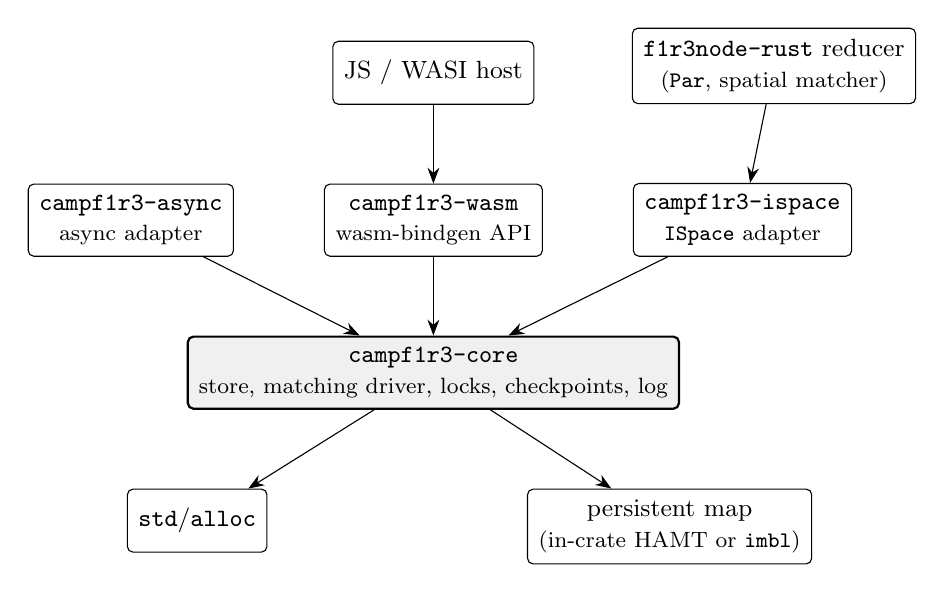
\begin{tikzpicture}[
  box/.style={draw,rounded corners=2pt,align=center,font=\small,minimum height=8mm,inner sep=4pt},
  core/.style={box,fill=black!6,thick},
  dep/.style={-{Stealth[length=2mm]},thin}]
\node[core,minimum width=58mm] (core) {\code{campf1r3-core}\\ \footnotesize store, matching driver, locks, checkpoints, log};
\node[box,above left=10mm and -6mm of core] (async) {\code{campf1r3-async}\\ \footnotesize async adapter};
\node[box,above=10mm of core] (wasm) {\code{campf1r3-wasm}\\ \footnotesize wasm-bindgen API};
\node[box,above right=10mm and -6mm of core] (isp) {\code{campf1r3-ispace}\\ \footnotesize \code{ISpace} adapter};
\node[box,above=10mm of isp,xshift=4mm] (node) {\code{f1r3node-rust} reducer\\ \footnotesize (\code{Par}, spatial matcher)};
\node[box,above=10mm of wasm] (js) {JS / WASI host};
\node[box,below=10mm of core,xshift=-30mm] (alloc) {\code{std}/\code{alloc}};
\node[box,below=10mm of core,xshift=30mm] (imbl) {persistent map\\ \footnotesize (in-crate HAMT or \code{imbl})};
\draw[dep] (async) -- (core); \draw[dep] (wasm) -- (core); \draw[dep] (isp) -- (core);
\draw[dep] (node) -- (isp); \draw[dep] (js) -- (wasm);
\draw[dep] (core) -- (alloc); \draw[dep] (core) -- (imbl);
\end{tikzpicture}
\end{center}

\begin{description}[nosep,leftmargin=1.5em,style=nextline]
\item[\code{campf1r3-core}] The store. It is synchronous, spawns no threads, uses no
  clocks and no randomness, and contains everything normative in
  Sections~\ref{sec:semantics}--\ref{sec:accounting}.
\item[\code{campf1r3-async}] A thin \code{async} facade over the core, for callers
  whose reducer is asynchronous. It \MUSTNOT{} add semantics.
\item[\code{campf1r3-wasm}] \code{wasm-bindgen} bindings exposing a byte-level
  instance of the core (Section~\ref{sec:wasmapi}).
\item[\code{campf1r3-ispace}] An implementation of \code{rspace++}'s \code{ISpace}
  for the \code{f1r3node} types, without history. It lives in the
  \code{f1r3node-rust} workspace, not in the \Camp{} repository, so the core never
  depends on \code{models}.
\end{description}

\subsection{The three parameters}

Following Remark~\ref{rem:factoring} and the FIP's outer/inner split, the core is
generic over three orthogonal choices:
\begin{center}
\begin{tabularx}{\linewidth}{@{}l>{\raggedright\arraybackslash}X>{\raggedright\arraybackslash}p{0.42\linewidth}@{}}
\toprule
Parameter & Role & Version 1 instances\\
\midrule
Key object & How channels address rows; what ``co-located'' means & \code{Flat} (required), \code{Path} (optional)\\
Collection & The bag at each row, for data and for continuations & \code{Bag} (required); \code{Set}, \code{Cell}, \code{Queue}, \code{Stack} (optional)\\
Matcher & $m$ and $\gamma$ of Section~\ref{sec:semantics} & caller-supplied; \code{ExactBytes} reference matcher\\
\bottomrule
\end{tabularx}
\end{center}
Each parameter is a trait, and the store is monomorphised over it, so choosing a
parameter costs no dynamic dispatch. A registry of named instances in the FIP
style (\code{rho:space:HashMapBagSpace}, \dots) belongs to the reducer's system
processes, not to the core.

%======================================================================
\section{Core traits}\label{sec:traits}

\subsection{Values supplied by the caller}

\begin{lstlisting}
/// 32-byte content hash. Computed once by the caller (for f1r3node:
/// Blake2b-256 of the canonical serialisation, already present in the
/// Produce/Consume event records). The core never hashes payloads.
#[derive(Copy, Clone, Eq, PartialEq, Ord, PartialOrd, Hash)]
pub struct Hash32(pub [u8; 32]);

pub trait Keyed {
    fn content_hash(&self) -> Hash32;
}

pub trait Channel: Keyed + Eq + Clone + Send + Sync + 'static {}
pub trait Datum:   Keyed + Clone + Send + Sync + 'static {}
pub trait Pattern: Clone + Send + Sync + 'static {}
pub trait Cont:    Keyed + Clone + Send + Sync + 'static {}
\end{lstlisting}

\begin{requirement}[Hash discipline]\label{req:hash}
The core \MUSTNOT{} compute a hash of $C$, $A$, $P$ or $K$ values. All keying,
sharding and ordering \MUST{} derive from \code{content\_hash}. Equal values
\MUST{} have equal hashes. Channel equality \MUST{} be decided by \code{Eq} after
hash equality, so a hash collision cannot merge two channels.
\end{requirement}

\begin{remark}
In \code{rspace++}, \code{shuffle\_with\_index} serialises every candidate with
\code{bincode} and hashes it with Blake2b on \emph{every} produce and consume,
and shard and stripe selection use \code{std}'s \code{DefaultHasher}, whose output
the standard library does not promise to keep stable. Requirement~\ref{req:hash}
removes the first cost entirely, and the second portability hazard.
\end{remark}

\subsection{Matcher}

\begin{lstlisting}
pub trait Matcher<P, A, K>: Send + Sync + 'static {
    /// m(p, a): Some(binding result) when a matches p.
    fn get(&self, p: &P, a: &A) -> Option<A>;
    /// gamma(k, bindings): the where-clause guard, run after every
    /// position has matched. Default: no guard.
    fn check_commit(&self, _k: &K, _bound: &[A]) -> bool { true }
}
\end{lstlisting}

This is \code{rspace++}'s \code{Match} trait verbatim, so the \code{f1r3node}
spatial matcher implements it unchanged.

\begin{requirement}[Matcher purity]\label{req:pure}
A matcher \MUST{} be a pure function of its arguments: deterministic, free of side
effects, and \MUSTNOT{} call back into the store. It is invoked while shard locks
are held (Section~\ref{sec:concurrency}); a re-entrant call would deadlock.
\end{requirement}

\subsection{Collections}

\begin{lstlisting}
pub trait Collection<T>: Clone + Default + Send + Sync {
    /// Insert an occurrence, returning its stable occurrence id.
    fn put(&mut self, item: T, key: OrderKey) -> OccId;
    fn remove(&mut self, id: OccId) -> Option<T>;
    /// Occurrences eligible to react, in the order the oracle sees them.
    /// A Bag yields all; a Queue yields only its head; a Cell its one item.
    fn eligible(&self) -> impl Iterator<Item = (OccId, &T)>;
    fn len(&self) -> usize;
    /// Algebraic laws the collection satisfies; see Section 9.
    const COMMUTATIVE: bool;
    const IDEMPOTENT: bool;
}
\end{lstlisting}

\subsection{Key object}

\begin{lstlisting}
pub trait KeyObject<C: Channel>: Send + Sync + 'static {
    /// Row key of a channel. Flat: its content hash.
    fn row_key(c: &C) -> Hash32;
    /// Rows that a send on `c` may meet, beyond its own row.
    /// Flat: none. Path: rows on the route to and below `c`.
    fn comparable_rows(c: &C) -> SmallRowSet;
}
\end{lstlisting}

%======================================================================
\section{Data structures}\label{sec:data}

\subsection{Rows and shards}

The store is an array of $S$ shards, $S$ a power of two fixed at construction
(default 64 on native targets, 1 on single-threaded WebAssembly). Row key $r$ lives
in shard $\sh(r)$, computed from the leading eight bytes of the key:
\[
  \sh(r) \;=\; \big(\mathrm{u64}_{\mathrm{le}}(r_{0..8}) \cdot \phi_{64}\big) \gg (64-\log_2 S),
\]
a Fibonacci hash with the fixed odd constant $\phi_{64}=\mathtt{0x9E3779B97F4A7C15}$.
This is total, platform independent, and cheap.

\begin{lstlisting}
// DC: Collection<DatumRec<A>>,  WC: Collection<ContRec<P, K>>
struct Shard<C, P, A, K, DC, WC> {
    lock:    Lock,                        // Section 7
    rows:    PMap<Hash32, Row<C, DC>>,
    groups:  PMap<GroupKey, GroupRow<C, P, K, WC>>,
    version: u64,                         // bumped on every write
}

struct Row<C, DC> {
    channel: C,
    data:    DC,                          // occurrences of DatumRec<A>
    joins:   SmallVec<[GroupKey; 2]>,     // J(c), ordinary and installed
}

struct GroupRow<C, P, K, WC> {
    channels:  SmallVec<[C; 2]>,          // ordered; repeats allowed
    waiting:   WC,                        // occurrences of ContRec<P, K>
    installed: SmallVec<[ContRec<P, K>; 1]>,
}
\end{lstlisting}

\code{PMap} is a persistent hash-array-mapped trie with structural sharing, so
cloning a shard's maps is a reference-count increment (Section~\ref{sec:checkpoint}).
\code{rspace++}'s current hot store already adopted this design
(\code{imbl::HashMap} per shard) to make soft checkpoints $O(S)$. \Camp{} keeps it.
A build feature \code{no-checkpoint} \MAY{} replace \code{PMap} with an ordinary
open-addressing map for callers that never checkpoint.

\subsection{Join groups and their home}

A group $g=(c_1,\dots,c_n)$ is keyed by
$\mathrm{GroupKey}(g)=H(\mathrm{hash}(c_1)\,\Vert\cdots\Vert\,\mathrm{hash}(c_n))$,
with $H$ a fixed 64-bit mixing function over the concatenated channel hashes
(computed by the core over hashes, not over channel values, which is consistent with
Requirement~\ref{req:hash}), and equality confirmed by comparing the channel
vectors. Order matters: patterns are positional.

The \code{GroupRow} lives in its \emph{home shard}, the least shard index among
$\{\sh(\mathrm{row}(c_i))\}$. Every member row records the group key in
\code{joins}. Hence:
\begin{itemize}[nosep]
\item $J(c)$ is read from $c$'s own row, under $c$'s own shard lock;
\item every shard holding any part of $g$ is in $\{\sh(\mathrm{row}(c_i))\}$, which is
      exactly the set a consume on $g$ locks.
\end{itemize}

Empty rows and empty group rows \MUST{} be removed eagerly, and a group key
\MUST{} be dropped from its member rows when the group row empties, so that the
store's size is proportional to its live contents.

\subsection{Records and order keys}

\begin{lstlisting}
struct DatumRec<A>    { value: A, persist: bool, key: OrderKey }
struct ContRec<P, K>  { patterns: SmallVec<[P; 2]>, cont: K,
                        persist: bool, peeks: PeekSet, key: OrderKey }

#[derive(Copy, Clone, Eq, PartialEq, Ord, PartialOrd)]
struct OrderKey { hash: Hash32, seq: u64 }
\end{lstlisting}

\code{hash} is the record's content hash. \code{seq} is an arrival number taken
from a per-space counter at commit time. \code{PeekSet} is a 64-bit mask; groups
wider than 64 channels are rejected. A \code{Bag} keeps its occurrences sorted by
\code{OrderKey} (a small sorted vector up to a threshold, a B-tree beyond it), so
iteration in oracle order costs nothing extra per operation.

\subsection{Matching strategy}\label{sec:matching}

Given a continuation $w$ at $g$ and the eligible occurrences at each position, the
driver searches for a candidate (Definition~\ref{def:candidate}).

\begin{description}[nosep,leftmargin=1.5em,style=nextline]
\item[\code{Greedy} (default).] For $i=1,\dots,n$ take the first eligible
  occurrence at $c_i$, in order-key order, not already chosen, that matches $p_i$.
  If some position fails, or the guard rejects, the continuation has no
  candidate. This is the strategy of \code{rspace++}'s
  \code{extract\_data\_candidates}.
\item[\code{Complete}.] Backtracking search over the same order, returning the
  first candidate in lexicographic order-key order, or none if none exists.
\end{description}

\begin{remark}[Greedy is incomplete]\label{rem:greedy}
Greedy search misses candidates in two situations. One is a channel repeated in a
group, with overlapping patterns, where the first choice at the earlier position
steals the only datum that fits the later one. The other is a guard that rejects the
greedy choice but would accept a later one. Under \code{Greedy},
Requirement~\ref{req:qui} holds only relative to the strategy: no redex
\emph{discoverable by greedy search} remains. \code{Complete} restores
Proposition~\ref{prop:qui} outright at a worst-case cost exponential in group
width; group widths are small in practice.
\end{remark}

\begin{decision}[Default matching strategy]
Default: \code{Greedy}, for behavioural parity with \code{rspace++}.
\code{Complete} is available per space. Review should decide whether guards
(\code{where} clauses) oblige \code{Complete} for groups that carry a guard.
\end{decision}
%======================================================================
\section{Operations}\label{sec:ops}

Every operation follows one skeleton: lock the footprint, consult the observer, search,
then either fire or store, log, and unlock. Every write happens after the last point
at which the operation can fail, so each operation is atomic.

\subsection{Mutating operations}

\paragraph{\code{produce(c, a, persist)}.}
\begin{enumerate}[nosep]
\item Compute $r=\code{row\_key}(c)$ and the datum occurrence $d$ with order key
      $(\code{a.content\_hash()},\ \bot)$; its \code{seq} is assigned at commit.
\item Lock the footprint $\{c\}\cup\bigcup J(c)$ (protocol~\ref{proto:produce}).
\item \code{observer.observe\_produce(\dots)?}.
\item For each group $g\in J(c)$ in ascending \code{GroupKey} order, for each
      continuation at $g$ --- installed ones first, then waiting ones in order-key
      order --- run the matching strategy with $d$ presented as the \emph{first}
      eligible occurrence at every position $i$ with $c_i=c$. Accept a candidate only
      if it uses $d$. The first accepted candidate is offered to the oracle, which in
      the \code{Deterministic} profile takes it.
\item If a candidate is taken: \code{observer.observe\_comm(\dots)?}; then remove the
      continuation if linear and not installed, remove each chosen stored datum that
      is linear and not at a peek position, log \textsf{Comm}, unlock, and return
      \code{Some(CommResult)}. $d$ is not stored.
\item Otherwise assign \code{seq}, insert $d$ into row $r$ (creating the row if
      needed), log \textsf{Produce}, unlock, and return \code{None}.
\end{enumerate}

\paragraph{\code{consume(g, patterns, k, persist, peeks)}.}
\begin{enumerate}[nosep]
\item Reject if $|g|\neq|\vec p|$, if $|g|=0$, if $|g|>64$, or if a peek index is out
      of range.
\item Lock the shards of $g$ in ascending order.
\item \code{observer.observe\_consume(\dots)?}.
\item Run the matching strategy for the new continuation over the stored data.
\item If a candidate is found: \code{observer.observe\_comm(\dots)?}; remove chosen
      linear non-peek data, log \textsf{Comm}, unlock, and return \code{Some}. The
      continuation is not stored.
\item Otherwise insert it into the group row in $g$'s home shard (creating the
      row and registering the group key in every member row if the group is new),
      log \textsf{Consume}, unlock, and return \code{None}.
\end{enumerate}

\paragraph{\code{install(g, patterns, k)}.} As \code{consume} with
\code{persist = true} and no peeks, except that a found candidate is an error
(\code{InstallWouldReact}) and the continuation goes to \code{installed}.

\subsection{Reads and administration}

\begin{center}
\begin{tabularx}{\linewidth}{@{}lX@{}}
\toprule
Operation & Contract\\
\midrule
\code{get\_data(c)} & Stored data at $c$, in order-key order. Takes $c$'s shard lock shared.\\
\code{get\_waiting(g)} & Waiting and installed continuations at $g$.\\
\code{get\_joins(c)} & $J(c)$ as channel vectors.\\
\code{remove\_all\_data(c)}, \code{remove\_all\_continuations(g)} & Administrative removal; logs nothing.\\
\code{clear()} & Empties the store, then re-applies installed continuations.\\
\code{export()} & All rows and groups, sorted by key; deterministic.\\
\code{soft\_checkpoint()}, \code{revert(cp)} & Section~\ref{sec:checkpoint}.\\
\code{take\_log()} & Section~\ref{sec:log}.\\
\bottomrule
\end{tabularx}
\end{center}

\begin{requirement}[Atomicity]
If an operation returns \code{Err}, the store's state, counters and log \MUST{} be
exactly as before the call.
\end{requirement}

\begin{remark}[Removing by index]
\code{rspace++}'s \code{ISpace} exposes \code{remove\_data\_at(channel, index)}. \Camp{}
does not expose positions: occurrence ids are stable, and the \code{ISpace} adapter
translates positions to ids against the order-key order it presented.
\end{remark}

%======================================================================
\section{Concurrency}\label{sec:concurrency}

\subsection{Model}

\Camp{} is a shared-memory store accessed by any number of caller threads. Every
mutating operation holds all locks covering its footprint from before its first read
to after its last write --- strict two-phase locking at shard granularity. With
Lemma~\ref{lem:indep} this gives the correctness criterion.

\begin{requirement}[Linearisability]\label{req:lin}
Every concurrent history of \Camp{} operations \MUST{} be linearisable with respect to
the sequential semantics of Section~\ref{sec:opsem}, with the linearisation point of
each operation being its commit under locks.
\end{requirement}

Two operations that hold a common shard are serialised by it. Two operations with
disjoint shard sets have disjoint footprints and therefore commute
(Lemma~\ref{lem:indep}), so any interleaving of them is equivalent to either serial
order. What remains is that the footprint an operation locks is its true footprint
at its linearisation point, and that locking cannot deadlock.

\subsection{Lock protocols}

Shards are totally ordered by index, and every protocol acquires locks in
ascending index order.

\begin{definition}[Consume and install]
Lock $L_g=\{\sh(\mathrm{row}(c))\mid c\in g\}$ in ascending order. $L_g$ depends
only on the arguments, so it is exact.
\end{definition}

\begin{definition}[Produce]\label{proto:produce}
Let $s_0=\sh(\mathrm{row}(c))$.
\begin{enumerate}[nosep]
\item Lock $s_0$. Read $J(c)$ and compute $L=\{s_0\}\cup\{\sh(\mathrm{row}(c'))\mid
      c'\in g,\ g\in J(c)\}$.
\item \emph{Fast path}: if $L=\{s_0\}$, proceed. This is the single-lock common case.
\item \emph{Ascending path}: if $\min L=s_0$, lock the rest of $L$ in ascending
      order while still holding $s_0$, and proceed.
\item \emph{Retry path}: otherwise release $s_0$, lock $L$ in ascending order,
      re-read $J(c)$ and recompute $L'$. If $L'\subseteq L$, proceed; otherwise
      release everything, set $L:=L\cup L'$, and repeat. After three rounds, lock
      every shard.
\end{enumerate}
\end{definition}

\begin{lemma}[Footprint stability]
While $s_0=\sh(\mathrm{row}(c))$ is held, $J(c)$ and the channel vector of every
group in $J(c)$ cannot change.
\end{lemma}
\begin{proof}
$J(c)$ changes only when a group containing $c$ is created (by \code{consume} or
\code{install} on that group) or removed (when its last continuation is removed by a
reaction or by administrative removal). Every such operation holds the shards of all
the group's channels, $s_0$ among them. A group's channel vector is fixed at creation.
\end{proof}

\begin{proposition}
The protocols are deadlock free, and each operation locks a superset of its footprint's
shards at its linearisation point.
\end{proposition}
\begin{proof}[Proof sketch]
All acquisitions are ascending: the ascending path acquires only indices above the
one it holds, and the retry path holds nothing when it starts a round. Stability
makes $L$ computed under $s_0$ exact, and in the retry path the recomputation is
made under $s_0$ as well. Livelock is bounded by the escalation to all shards.
\end{proof}

\subsection{Lock implementation by target}

\begin{center}
\begin{tabularx}{\linewidth}{@{}lX@{}}
\toprule
Build & \code{Lock}\\
\midrule
native & \code{std::sync::Mutex<()>} per shard, with shared reads through snapshots (below). A \code{parking\_lot} feature \MAY{} substitute.\\
\code{wasm32}, no atomics & A zero-cost cell. The type is \code{Sync} only under \code{cfg(not(target\_feature = "atomics"))}, where no second thread can exist.\\
\code{wasm32} + atomics, \code{wasip1-threads} & \code{std::sync::Mutex}, which uses \code{memory.atomic.wait32}.\\
\bottomrule
\end{tabularx}
\end{center}

\begin{requirement}[Browser main thread]
In builds with atomics, a contended lock blocks with \code{Atomics.wait}, which
browsers forbid on the main thread. Blocking operations \MUST{} be documented as
worker-only, and the core \MUST{} provide \code{try\_}-prefixed variants that return
\code{WouldBlock} instead of waiting.
\end{requirement}

\begin{requirement}[No threads, no clocks, no randomness]
The core \MUSTNOT{} spawn threads, read clocks (\code{std::time::Instant} panics on
\code{wasm32-unknown-unknown}), or draw randomness. Metrics timing, if any, \MUST{}
go through an optional caller-supplied clock trait.
\end{requirement}

\subsection{Reads without writers' locks}

Read operations take the relevant shard lock only long enough to clone the shard's
persistent maps, then read the clone with no lock held. For \code{get\_data} this is
a single reference-count increment.

\subsection{Optional optimistic matching}

Matching runs under locks, and a spatial matcher can be expensive, so a long match
stalls its shards. The feature \code{optimistic} \MAY{} be enabled:
\begin{enumerate}[nosep]
\item snapshot the footprint shards (clone maps and record each shard's
      \code{version});
\item run the matching strategy on the snapshot, with no lock held;
\item lock the footprint, and commit the snapshot's decision if every footprint
      shard's version is unchanged; otherwise discard it and run pessimistically.
\end{enumerate}
Validation is per shard, and therefore conservative. The result is still strict 2PL
at commit, so Requirement~\ref{req:lin} is unaffected.

%======================================================================
\section{Checkpoints and the event log}\label{sec:checkpoint}

\subsection{Soft checkpoints}

\code{soft\_checkpoint()} locks every shard in ascending order, clones each shard's
persistent maps ($O(S)$ reference-count increments), records the \code{seq} counter
and the log watermark, and releases. \code{revert(cp)} locks every shard, replaces
the maps, restores the counter, truncates the log to the watermark, re-applies the
installed continuations, and releases. Both are global quiescent points.

\begin{requirement}
\code{soft\_checkpoint} \MUST{} cost $O(S)$ time and allocation, independent of the
number of stored records.
\end{requirement}

There are no hard checkpoints. A caller that needs a state root \MAY{} enable
\code{digest}, which folds a caller-supplied hasher over \code{export()} in key
order. Such roots are \Camp{} roots, not \code{rspace++} history roots.

\subsection{Event log}\label{sec:log}

With the feature \code{log}, each committing mutation appends one event, stamped with
a sequence number drawn from a per-space \code{AtomicU64} while its locks are held, to
a buffer in its home shard (the least shard it holds):
\[
  \textsf{Produce}(h_c,h_a,\pi)\qquad
  \textsf{Consume}(\vec h_c,h_k,\pi)\qquad
  \textsf{Comm}\big(\textsf{Consume},\ \overrightarrow{\textsf{Produce}},\ E\big).
\]
All hashes are caller-supplied content hashes.

\code{take\_log()} reads the counter as a watermark $M$, then visits the shards in
ascending order, draining each buffer's events with sequence number below $M$, and
finally sorts the result by sequence number. An operation whose number is below $M$
was stamped while holding its home shard, before $M$ was read, so the drain of that
shard waits for it and sees the event. An operation that takes a shard after the
drain passed it is stamped after $M$ was read, so its number is at least $M$. The
log therefore needs no global mutex, and its order is a valid linearisation order.

%======================================================================
\section{Determinism and replay}\label{sec:determinism}

The source paper leaves the pairing of sends with receives as a relation. A store
has to choose. \Camp{} isolates the choice in the oracle $\omega$ and offers three
profiles.

\begin{description}[nosep,leftmargin=1.5em,style=nextline]
\item[\code{Free}.] The oracle takes whatever candidate the strategy finds first,
  and collections \MAY{} iterate in arrival order without sorting. Correct up to
  resource bisimilarity; fastest.
\item[\code{Deterministic} (default).] Candidates are explored in the canonical
  order of Section~\ref{sec:ops}: groups by \code{GroupKey}, installed before waiting,
  continuations and data by \code{OrderKey}. The first candidate wins.
\item[\code{Replay}.] \code{rig(log)} loads an expected multiset of \textsf{Comm}
  events. The oracle accepts a candidate only if the continuation hash and datum hashes
  match an expected \textsf{Comm}, which is then decremented. An operation that would
  otherwise react with no matching expectation stores its record instead.
  \code{check\_replay()} fails if expectations remain. This is \code{IReplayRSpace}'s
  contract. Under \code{Replay}, quiescence holds only relative to the expectations:
  a record stored while awaiting its recorded partner may coexist with an unrecorded
  match.
\end{description}

\begin{requirement}[Deterministic profile]\label{req:det}
For a serial sequence of calls with equal arguments, in the \code{Deterministic}
profile, results, \code{export()}, and the log \MUST{} be bit-identical across
targets, pointer widths, shard counts and thread counts. For a concurrent execution,
they \MUST{} equal those of the serial execution in log order.
\end{requirement}

Shard count does not affect determinism, because order keys and group keys are derived
from content hashes rather than shard placement.

\begin{remark}[Relation to \code{rspace++} ordering]
\code{rspace++} orders candidates by the Blake2b hash of their \code{bincode} encoding,
then by position. \Camp{}'s \code{OrderKey} is the same shape, with the hash supplied
by the caller and the position replaced by a stable arrival number. Whether the two
orders agree on every workload is Obligation~\ref{ob:diff}.
\end{remark}

\begin{decision}[Replay compatibility with f1r3node]\label{dec:replay}
Must \Camp{} replay logs produced by \code{rspace++}, and produce logs that
\code{rspace++} replays? Default in this draft: the core guarantees
Requirement~\ref{req:det} and the \code{Replay} profile over caller-supplied hashes.
Bit-compatibility with \code{rspace++} event hashes and candidate order is a
conformance target of the \code{campf1r3-ispace} adapter, validated by differential
testing, not a core requirement.
\end{decision}

%======================================================================
\section{Cost accounting}\label{sec:accounting}

In the cost-accounted rho calculus, a communication is where resources are debited:
located token stacks travel as data, and signature-keyed entries are simply further
channels. The COMM is also the witness of RSpace's distributive law. \Camp{} therefore
hooks accounting exactly at the zip and nowhere else.

\begin{lstlisting}
pub trait Observer<C, P, A, K>: Send + Sync + 'static {
    fn observe_produce(&self, c: &C, a: &A, persist: bool) -> Result<(), Abort>;
    fn observe_consume(&self, g: &[C], ps: &[P], k: &K,
                       persist: bool, peeks: PeekSet) -> Result<(), Abort>;
    fn observe_comm(&self, k: &K, k_persist: bool,
                    data: &[(&A, bool)]) -> Result<(), Abort>;
}
\end{lstlisting}

This mirrors \code{rspace++}'s \code{RSpaceAccountingObserver}.

\begin{requirement}[Accounting hooks]
Observers are called under the operation's locks, before any write. An \code{Err}
aborts the operation under the atomicity requirement. Observers \MUSTNOT{} call the
store, but \MAY{} mutate their own budget, which \SHOULD{} be lock-free (for example
an \code{AtomicU64}). Any policy about which data may match, such as
\code{rspace++}'s refusal to match data carrying a cost stack, belongs to the
matcher, not to the store.
\end{requirement}
%======================================================================
\section{Storage variants}\label{sec:variants}

\subsection{Collections}

\begin{center}
\begin{tabularx}{\linewidth}{@{}lccX@{}}
\toprule
Collection & Comm. & Idem. & Semantics and caveat\\
\midrule
\code{Bag} & yes & no & Multiset. The only collection under which Proposition~\ref{prop:hom} holds. Required.\\
\code{Set} & yes & yes & Re-inserting an equal record (same content hash) is a no-op. Denotes $\mathcal P_{\mathrm{fin}}$ rather than $\Mfin$, so $x!(0)\mid x!(0)\equiv x!(0)$ at that channel.\\
\code{Cell} & -- & -- & At most one datum and one continuation; a second \code{put} is an error (\code{CellOccupied}).\\
\code{Queue} & no & no & FIFO; only the head is eligible. Parallel composition at the channel stops commuting.\\
\code{Stack} & no & no & LIFO; only the top is eligible. Same caveat.\\
\bottomrule
\end{tabularx}
\end{center}

\begin{requirement}[Non-commutative collections]
A space whose collection has \code{COMMUTATIVE = false} \MUST{} be constructed with
the \code{Seq} qualifier (below). Its determinism depends on caller-agreed arrival
order, which \Camp{} records but cannot establish across nodes.
\end{requirement}

\subsection{Key objects}

\code{Flat} keys each row by its channel's content hash. It is required, and it is
reading~(0)/(1) of \emph{Paths are Subspaces}: every theorem of the flat model transfers
verbatim.

\code{Path} (optional) takes $C=\mathrm{Name}^{*}$ and implements \emph{cut-triggered
subspace reaction}. The rows are a trie, and a send on $p$ may meet a receive on any
path comparable with $p$ in the prefix order. The two dual rules are:
\begin{description}[nosep,leftmargin=1.5em]
\item[\textsc{Out-deep}] a receive on $p_1$ meets a send on $p_2=p_1\cdot w$; the
  receiver binds the sealed, still-located sub-RSpace $@(w\rhd Q)$.
\item[\textsc{In-deep}] a send on $p_2$ meets a receive on $p_1=p_2\cdot w$; the cut
  unpacks into a fresh cut $\mathsf{for}(y\leftarrow w)P\mid Q$, which \Camp{} returns
  to the caller as a comm result of kind \code{Descend}, not as a store mutation.
\end{description}
No-implicit-interaction (Remark~\ref{rem:noimplicit}) is preserved: the trie never
reacts internally, and footprints become ``the row and its comparable rows'', which
\code{KeyObject::comparable\_rows} supplies to the lock protocol.

\begin{decision}[Path semantics]
The FIP's PathMap example composes stores upward, so a send is also a send on every
prefix, and it has no \textsc{In-deep} rule. \emph{Paths are Subspaces} insists on
no implicit interaction and has both rules. Default: implement the latter, and
reconcile the FIP before \code{Path} is stabilised.
\end{decision}

\subsection{Qualifiers}

The FIP's qualifiers are accepted at construction.
\begin{description}[nosep,leftmargin=1.5em]
\item[\code{Default}] Concurrent. Included in \code{export} and \code{digest}.
\item[\code{Temp}] Concurrent. Excluded from \code{export} and \code{digest}, so the
  caller does not persist it.
\item[\code{Seq}] As \code{Temp}. The FIP's static restrictions (the name is never sent
  and is used in at most one sequential process) are enforced by the reducer. \Camp{}
  \MAY{} additionally assert single-threaded access in debug builds.
\end{description}

%======================================================================
\section{Portability and WebAssembly}\label{sec:wasm}

\subsection{Targets}

\begin{center}
\begin{tabularx}{\linewidth}{@{}>{\raggedright\arraybackslash}p{0.34\linewidth}cX@{}}
\toprule
Target & Level & Notes\\
\midrule
\code{x86\_64}/\code{aarch64} Linux, macOS & \MUST & Reference platform.\\
\code{wasm32-unknown-unknown} & \MUST & Single-threaded; $S=1$; zero-cost locks.\\
\code{wasm32-unknown-unknown} with atomics & \SHOULD & Needs \code{-C target-feature=+atomics,+bulk-memory}, nightly \code{build-std}, and a host serving COOP/COEP headers for \code{SharedArrayBuffer}; workers supplied by the host.\\
\code{wasm32-wasip1-threads} & \SHOULD & Stable target; for wasmtime and similar non-browser hosts.\\
\bottomrule
\end{tabularx}
\end{center}

\begin{requirement}[Portable arithmetic]
Identifiers, sequence numbers, counters and sizes that are observable or logged
\MUST{} be \code{u64} or narrower fixed-width types, never \code{usize}, so that 32-bit
WebAssembly and 64-bit native builds agree bit for bit.
\end{requirement}

\subsection{Dependencies}\label{sec:deps}

\begin{requirement}[Dependency allowlist]
\code{campf1r3-core} \MUST{} build with only \code{std} (or \code{alloc}) and, at most,
\code{smallvec} and a persistent-map crate (\code{imbl}, or an in-crate HAMT). Optional
features \MAY{} add \code{parking\_lot}. It \MUSTNOT{} depend, directly or
transitively, on \code{tokio}, \code{rayon}, \code{heed} or any C library,
\code{getrandom}, \code{serde}, \code{bincode}, or any crate of the
\code{f1r3node-rust} workspace.
\end{requirement}

Serialisation is excluded on purpose: the caller already owns a canonical encoding and
supplies its hashes. An optional \code{serde} feature \MAY{} derive encodings for
\code{export} snapshots.

\subsection{The WebAssembly API}\label{sec:wasmapi}

\code{campf1r3-wasm} instantiates the core at
$C=A=K=\code{Bytes}$, with patterns drawn from a small reference language (exact
bytes, prefix, wildcard) and the \code{ExactBytes} matcher. Content hashes are
computed at the boundary by a host-provided function or by the bundled
\code{blake3} feature. This makes \Camp{} usable, and testable, in a browser before the
parser and normaliser are ported. A rholang instance replaces the reference matcher
once those components are available.

\begin{lstlisting}
#[wasm_bindgen] impl Space {
    pub fn new(config: JsValue) -> Result<Space, JsError>;
    pub fn produce(&self, ch: &[u8], data: &[u8], persist: bool)
        -> Result<Option<CommResult>, JsError>;
    pub fn consume(&self, chans: Array, pats: Array, cont: &[u8],
                   persist: bool, peeks: u64) -> Result<Option<CommResult>, JsError>;
    pub fn try_produce(/* same */) -> Result<TryResult, JsError>; // WouldBlock
    pub fn checkpoint(&self) -> Checkpoint;
    pub fn revert(&self, cp: Checkpoint) -> Result<(), JsError>;
}
\end{lstlisting}

%======================================================================
\section{Rust interface}\label{sec:api}

\begin{lstlisting}
pub struct Space<C, P, A, K, M, O, DC, WC, KO> { /* shards, config */ }

pub struct Config {
    pub shards: u32,                 // power of two
    pub profile: Profile,            // Free | Deterministic | Replay
    pub strategy: Strategy,          // Greedy | Complete
    pub qualifier: Qualifier,        // Default | Temp | Seq
}

pub struct CommResult<C, P, A, K> {
    pub cont: K, pub cont_persist: bool,
    pub channels: SmallVec<[C; 2]>, pub patterns: SmallVec<[P; 2]>,
    pub bound: SmallVec<[Bound<A>; 2]>,   // (binding, removed datum, persist)
    pub peeks: PeekSet,
    pub kind: CommKind,                   // Apply | Descend (Path only)
}

impl<...> Space<...> {
    pub fn new(cfg: Config, matcher: M, observer: O) -> Self;
    pub fn produce(&self, c: C, a: A, persist: bool)
        -> Result<Option<CommResult<C, P, A, K>>, SpaceError>;
    pub fn consume(&self, g: &[C], ps: &[P], k: K, persist: bool,
                   peeks: PeekSet) -> Result<Option<CommResult<C, P, A, K>>, SpaceError>;
    pub fn install(&self, g: &[C], ps: &[P], k: K) -> Result<(), SpaceError>;
    // try_produce / try_consume, reads, admin, checkpoints, log, replay ...
}
\end{lstlisting}

All methods take \code{\&self}, and \code{Space} is \code{Send + Sync} whenever its type
parameters are. The error type is a closed enumeration: \code{Aborted}
(observer), \code{ArityMismatch}, \code{GroupTooWide}, \code{InstallWouldReact},
\code{CellOccupied}, \code{WouldBlock}, \code{ReplayMismatch}, and
\code{QualifierViolation}.

%======================================================================
\section{Integration with f1r3node}\label{sec:integration}

\code{campf1r3-ispace} instantiates the core at \code{Par}, \code{BindPattern},
\code{ListParWithRandom}, \code{TaggedContinuation}, with the reducer's spatial
\code{Matcher} and a bridge from \code{RSpaceAccountingObserver} to \code{Observer}.
Content hashes are the Blake2b-256 hashes that \code{rspace++} already computes for its
\code{Produce} and \code{Consume} events.

\begin{center}
\begin{tabularx}{\linewidth}{@{}l>{\raggedright\arraybackslash}X@{}}
\toprule
\code{ISpace} method & \Camp{}\\
\midrule
\code{produce}, \code{consume}, \code{install} & Direct.\\
\code{get\_data}, \code{get\_waiting\_continuations}, \code{get\_joins} & Direct.\\
\code{remove\_data\_at}, \code{remove\_all\_*} & Position translated to occurrence id.\\
\code{create\_soft\_checkpoint}, \code{revert\_to\_soft\_checkpoint} & Direct.\\
\code{take\_event\_log} & \code{take\_log}, events re-encoded to \code{rspace++} records.\\
\code{rig}, \code{rig\_and\_reset}, \code{check\_replay\_data}, \code{is\_replay} & \code{Replay} profile.\\
\code{set\_accounting\_observer} & Observer bridge (swappable through an \code{ArcSwap}).\\
\code{to\_map} & \code{export}.\\
\code{create\_checkpoint}, \code{reset}, \code{get\_root} & Unsupported unless \code{digest}; roots are not \code{rspace++} roots.\\
\bottomrule
\end{tabularx}
\end{center}

The adapter is what makes differential testing against \code{rspace++} possible, and
lets the reducer run over \Camp{} for evaluation paths that do not need history, such as
exploratory deploys, local evaluation, and tests.

%======================================================================
\section{Performance}\label{sec:perf}

\subsection{Complexity}

Let $n_c=|D(c)|$, $j=|J(c)|$, $w_g$ the number of continuations at $g$, $\ell=|g|$,
$\mu$ the cost of one matcher call, and $S$ the shard count.

\begin{center}
\begin{tabular}{@{}lll@{}}
\toprule
Operation & Locks & Time (Greedy, excluding observer)\\
\midrule
produce, no joins on $c$ & 1 & $O(\log n_c)$ insert\\
produce, with joins & $\le\ell\cdot j$ shards & $O\big(\sum_{g\in J(c)} w_g\,\ell\,\mu\cdot\max_i n_{c_i}\big)$ worst case\\
consume on $g$ & $\le\ell$ & $O(\ell\,\mu\cdot\max_i n_{c_i})$\\
get\_data & 1, briefly & $O(1)$ snapshot\\
soft\_checkpoint & $S$, briefly & $O(S)$\\
take\_log & $S$, in turn & $O(e\log e)$ for $e$ events\\
\bottomrule
\end{tabular}
\end{center}

The worst cases are dominated by $\mu$, the spatial matcher. The store's own overhead
per matcher call is $O(1)$ and \MUSTNOT{} include hashing, serialisation or
allocation of payloads.

\subsection{Benchmarks and targets}

The benchmark suite \MUST{} include:
\begin{enumerate}[nosep]
\item single-channel produce/consume ping-pong (fast path);
\item $N$ disjoint channel pairs across $T$ threads, for scaling;
\item a hot contended channel with $T$ threads;
\item joins of width 2 and 4 with overlapping members;
\item persistent receive with a produce storm (the re-issue loop);
\item checkpoint and revert every $k$ operations;
\item the \code{rspace++} benches \code{bench\_par\_branches\_channel\_reuse} and
      \code{bench\_par\_reducer}, run through the adapter.
\end{enumerate}

\begin{requirement}[Performance targets]
Absolute targets are set after baseline measurement of \code{rspace++}'s hot store on
the reference platform, with the \code{rspace++} history layer disabled. Version~1
\MUST{} not regress against that baseline on any benchmark, \SHOULD{} scale benchmark~2
to within 80\% of linear up to $\min(S,\text{cores})$, and \MUST{} run benchmarks 1 and 6
on \code{wasm32-unknown-unknown} within a small constant factor of native. That factor
is to be fixed at review.
\end{requirement}

%======================================================================
\section{Conformance and testing}\label{sec:testing}

\begin{enumerate}[nosep]
\item \textbf{Reference model.} A separate, deliberately naive, single-threaded
      implementation of Section~\ref{sec:opsem} (vectors of records, exhaustive
      candidate enumeration) of a few hundred lines. It is the executable
      specification.
\item \textbf{Model-based property tests.} Random operation sequences run against
      the core and the reference model, comparing results, \code{export()}, and
      quiescence after every step (\code{Complete} strategy), or discoverable
      quiescence (\code{Greedy}).
\item \textbf{Linearisability checking.} Concurrent histories recorded under stress
      are checked against the reference model with a Wing--Gong style checker.
\item \textbf{Lock-protocol model checking.} The produce protocol and log drain are
      checked with \code{loom}, which \code{f1r3node-rust} already uses under
      \code{formal/loom}.
\item \textbf{Cross-target determinism.} The same seeded operation traces run
      natively and under \code{wasm-bindgen-test}, with \code{export()} and logs
      compared bit for bit (Requirement~\ref{req:det}).
\item \textbf{Differential testing.} The \code{rspace++} test suite runs through
      \code{campf1r3-ispace}, and randomised reducer workloads are compared against
      \code{rspace++} up to resource bisimilarity, and exactly where
      Decision~\ref{dec:replay} demands it.
\end{enumerate}

\begin{obligation}[Differential agreement]\label{ob:diff}
Establish, by the differential suite, whether \code{Deterministic} candidate order
agrees with \code{rspace++}'s, and characterise any divergence.
\end{obligation}

\begin{obligation}[Greedy parity]
Confirm that \code{Greedy} as specified coincides with \code{rspace++}'s
\code{extract\_data\_candidates} on every workload, including repeated channels
within a group, peeks, and guards.
\end{obligation}

%======================================================================
\section{Summary of obligations and open decisions}\label{sec:open}

\begin{center}
\begin{tabularx}{\linewidth}{@{}lX@{}}
\toprule
Item & Status in this draft\\
\midrule
Obligation~\ref{ob:comm} & Comm rules as single COMM steps --- the bialgebra obligation extended to joins, patterns, persistence, peeks, guards. Open.\\
Obligation~\ref{ob:diff} & Candidate-order agreement with \code{rspace++}. By test.\\
Greedy parity & By test.\\
Default strategy & \code{Greedy}; guarded groups may require \code{Complete}.\\
Replay compatibility & Core: deterministic and \code{Replay} over caller hashes; bit-compatibility is an adapter target.\\
Path semantics & \emph{Paths are Subspaces} over the FIP example, pending reconciliation.\\
Performance constants & Fixed after baseline measurement.\\
\bottomrule
\end{tabularx}
\end{center}

\subsection*{Roadmap}
\begin{enumerate}[nosep]
\item Reference model and property-test harness.
\item Core with \code{Flat} and \code{Bag}, \code{Greedy} and \code{Complete},
      pessimistic locking, \code{Deterministic} profile, soft checkpoints.
\item \code{wasm32-unknown-unknown} build and byte-level API; cross-target
      determinism tests.
\item Event log, \code{Replay} profile, observer; \code{campf1r3-ispace} and
      differential testing against \code{rspace++}.
\item Threads on WebAssembly; the \code{optimistic} feature; benchmarks and
      performance targets.
\item Optional collections, \code{Path} key object, and qualifiers.
\end{enumerate}

\end{document}
